\subsection{Applicazione dell'algoritmo di compressione ad alcune immagini}
Una volta portato a termine lo sviluppo di questo progetto, sono stati effettuati degli esperimenti su alcune immagini per poter osservare a livello visivo i risultati ottenuti operando sulle matrici. In seguito sono mostrate due figure di esempio che mostrano il confronto tra immagine originale e processata. \\\\
\begin{figure}[H]
    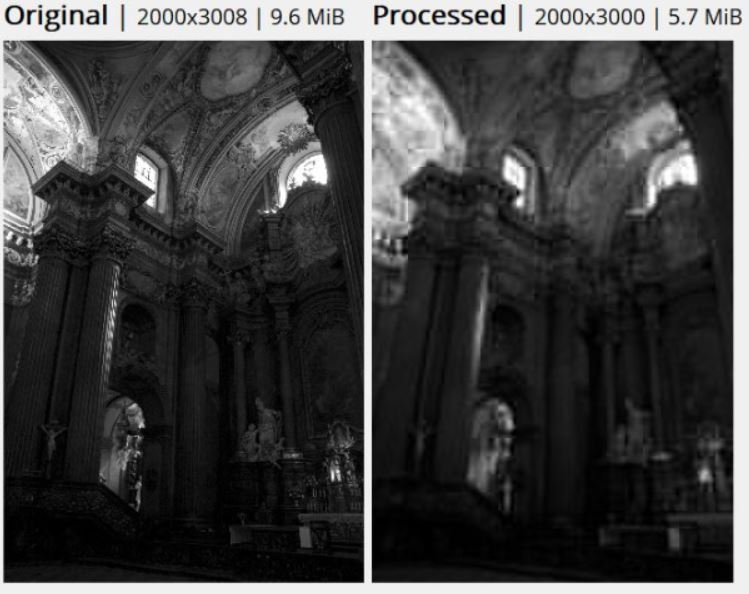
\includegraphics[scale=0.5]{ex1_cathedral}\centering
    \caption{Esempio 1 - Compressione con F=100, d=5}\label{fig:ex1_cathedral}
\end{figure}

\begin{figure}[H]
    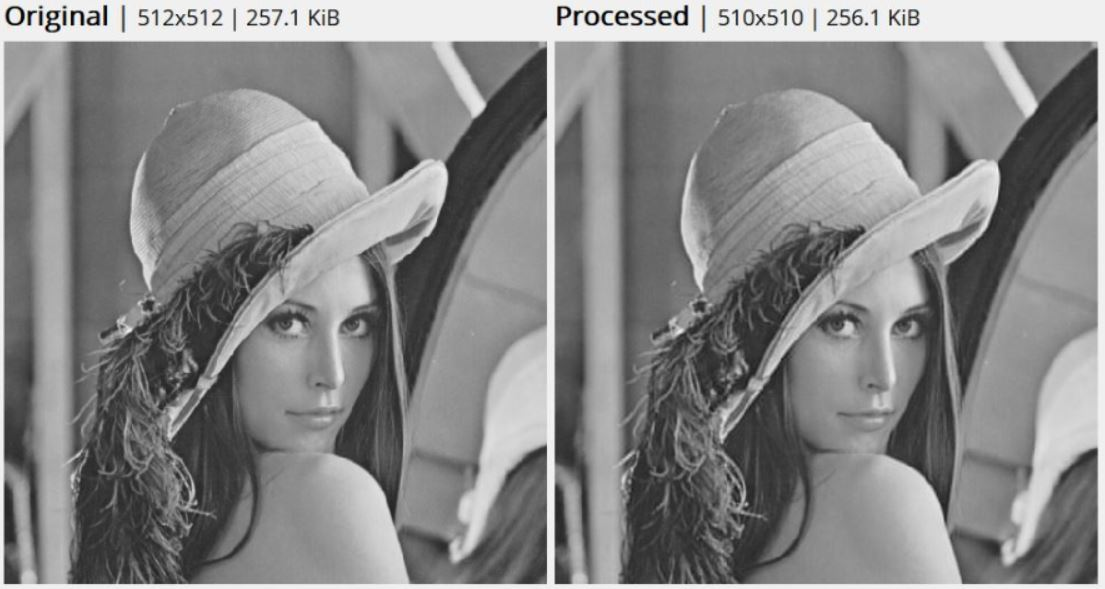
\includegraphics[scale=0.5]{ex2_woman}\centering
    \caption{Esempio 2 - Compressione con F=15, d=10}\label{fig:ex2_woman}
\end{figure}

Nel caso della figura \ref{fig:ex1_cathedral} è stata impostata su un'immagine 2000x3008 la dimensione di 100 per i macro-blocchi (F) e il valore di 5 (d) come soglia di taglio delle frequenze. Questa configurazione porta al raggruppamento della matrice originale in 30 righe e 20 colonne\footnote{Si ricorda che i pixels in eccesso rispetto ai blocchi vengono direttamente scartati causando un eventuale ridimensionamento dell'immagine} di blocchi 100x100. La soglia di taglio bassa porta all'eliminazione di gran parte delle frequenze generando una forte compressione che abbassa di molto la qualità dell'immagine originale.\\
Nella figura \ref{fig:ex2_woman}, invece, vediamo un esempio di minor compressione. In questo caso vengono utilizzati su un'immagine 512x512 i parametri 15 per la grandezza dei macro-blocchi e 10 per la soglia di taglio, portando alla formazione di una matrice quadrata con righe e colonne divise in 34 blocchi. Rispetto a prima la porzione di frequenze tagliate è proporzionalmente molto più contenuta. Nel confronto si può osservare che l'immagine processata non presenta rilevanti differenze visive rispetto all'originale.\\\\

Un'ulteriore sperimentazione è stata quella di far variare sulla stessa immagine prima il parametro della dimensione dei blocchi mantenendo fissa la soglia di taglio, per poi fare il viceversa. L'immagine su cui sono state svolti i test è quella in figura \ref{fig:original_deer}.\\

\begin{figure}[H]
    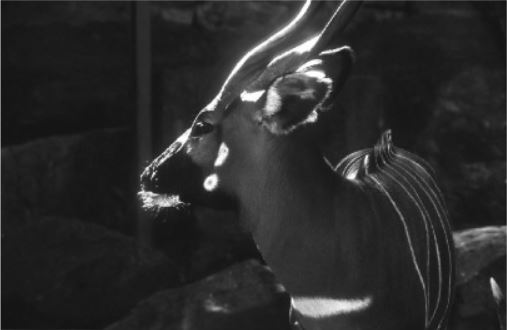
\includegraphics[scale=0.6]{original_deer}\centering
    \caption{Immagine originale sequenza esempi - 1011x661 | 1.9Mib}\label{fig:original_deer}
\end{figure}

La sequenza delle figure \ref{fig:fixedD1_deer}-\ref{fig:fixedD2_deer}-\ref{fig:fixedD3_deer} mostra i risultati ottenuti fissando a 10 la soglia di taglio delle frequenze e facendo variare la dimensione dei blocchi tra i valori 10-50-100. Come si può vedere la qualità dell'immagine compressa va peggiorando, in quanto l'aumentare della dimensione dei blocchi non seguito da un aumento anche della soglia di taglio porta a scartare per ogni blocco una porzione sempre più ampia di frequenze. Un'osservazione che si può fare è che, dovendo processare meno blocchi, anche i tempi di esecuzione si abbassano assieme alla qualità. Le immagini sono state computate rispettivamente in 1.110s, 0.325s e 0.265s.\\

\begin{figure}[H]
    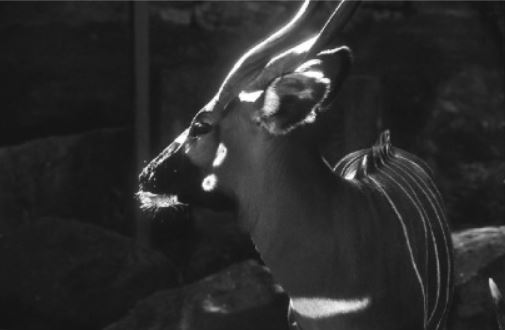
\includegraphics[scale=0.6]{fixedD1_deer}\centering
    \caption{Esempio fissata soglia - F=10, d=10; 1010x660 | 653.3Kib | 1.110s}\label{fig:fixedD1_deer}
\end{figure}
\begin{figure}[H]
    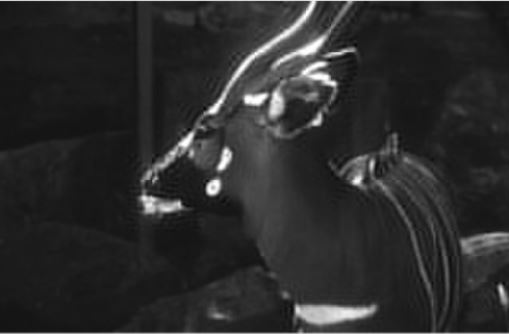
\includegraphics[scale=0.6]{fixedD2_deer}\centering
    \caption{Esempio fissata soglia - F=50, d=10; 1000x650 | 635.8Kib | 0.325s}\label{fig:fixedD2_deer}
\end{figure}
\begin{figure}[H]
    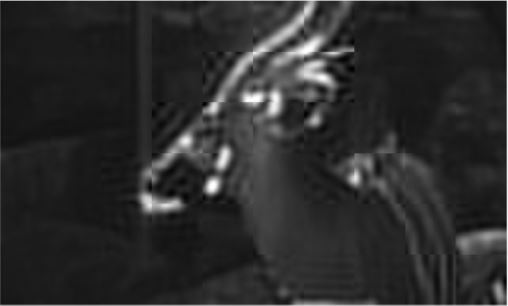
\includegraphics[scale=0.6]{fixedD3_deer}\centering
    \caption{Esempio fissata soglia - F=100, d=10; 1000x600 | 587.0Kib | 0.265s}\label{fig:fixedD3_deer}
\end{figure}

Con la sequenza di figure \ref{fig:fixedF1_deer}-\ref{fig:fixedF2_deer}-\ref{fig:fixedF3_deer} sono mostrati i risultati ottenuti fissando a 50 la dimensione dei blocchi e facendo variare la soglia di taglio tra i valori 1-10-30. In questo caso si può notare che il comportamento è opposto rispetto a quello della precedente sequenza di immagini. La causa del miglioramento della qualità è che per ogni blocco vengono preservate sempre più frequenze.\\
Contrariamente a quanto succede in precedenza, in questo caso i tempi impiegati restano molto simili tra loro perché il numero di blocchi da processare resta il medesimo in tutti e tre i casi. Le immagini sono state processate rispettivamente in 0.320s, 0.321s e 0.330s.

\begin{figure}[H]
    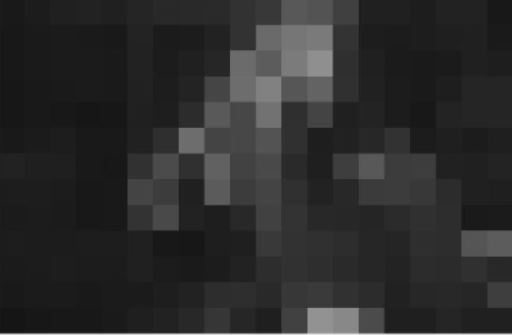
\includegraphics[scale=0.6]{fixedF1_deer}\centering
    \caption{Esempio fissata soglia - F=50, d=1; 1000x650 | 635.8Kib | 0.320s}\label{fig:fixedF1_deer}
\end{figure}
\begin{figure}[H]
    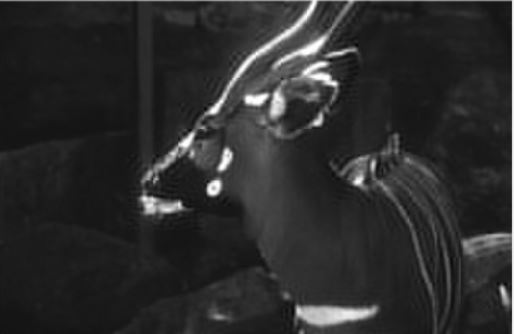
\includegraphics[scale=0.6]{fixedF2_deer}\centering
    \caption{Esempio fissata soglia - F=50, d=10; 1000x650 | 635.8Kib | 0.321s}\label{fig:fixedF2_deer}
\end{figure}
\begin{figure}[H]
    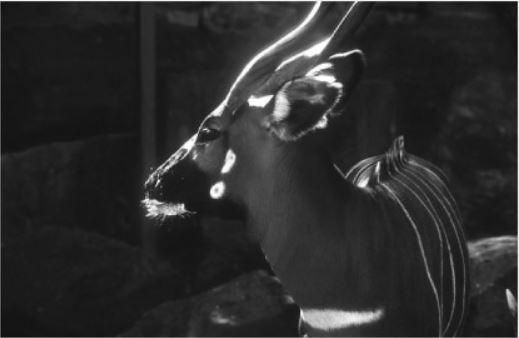
\includegraphics[scale=0.6]{fixedF3_deer}\centering
    \caption{Esempio fissata soglia - F=50, d=30; 1000x650 | 635.8Kib | 0.330s}\label{fig:fixedF3_deer}
\end{figure}
